\documentclass[11pt]{article}
\usepackage{amsmath,amsthm,amssymb,mathtools,tikz,epsfig,enumerate}
\usepackage{hyperref,titling,titlesec,pdfpages,setspace,fancyhdr,multicol,appendix}
\usepackage[numbers]{natbib}
\usepackage[margin=1in]{geometry} 

% formatting
%\setlength{\parskip}{2ex}
%\setlength{\parindent}{0pt}

% statement environment
\newtheorem{thm}{Theorem}[section]
\newtheorem{prop}[thm]{Proposition}
\newtheorem{lem}[thm]{Lemma}
\newtheorem{cor}[thm]{Corollary}
 
\theoremstyle{definition}
\newtheorem{defn}[thm]{Definition}
\newtheorem{prob}[thm]{Problem}
\newtheorem{eg}[thm]{Example}
 
\theoremstyle{remark}
\newtheorem{rem}[thm]{Remark}

% shorthand notations
\newcommand{\E}{\mathbb{E}} % expectation
\renewcommand{\P}{\mathbb{P}} % probability
\newcommand{\I}{\mathbb{I}} % indicator
\newcommand{\F}{\mathcal{F}} % filtration
\DeclarePairedDelimiter{\abs}{\lvert}{\rvert} % absolute value, or cardinality
\DeclarePairedDelimiter{\norm}{\lVert}{\rVert} % norm
\newcommand{\ts}{\textstyle}
\DeclareMathOperator{\esssup}{ess\, sup}
\newcommand*{\remaend}{\hfill\text{$\diamond$}}
\newcommand{\close}{\hspace*{\fill}$\diamond$}
\newcommand{\closeEqn}{\tag*{$\diamond$}}
\newcommand{\de}{\,\mathrm{d}}

\let\oldthebibliography=\thebibliography
\let\endoldthebibliography=\endthebibliography
\renewenvironment{thebibliography}[1]{%
\begin{oldthebibliography}{#1}%
\setlength{\baselineskip}{.8em}
\linespread{.8}
\small 
\setlength{\parskip}{0ex}%
\setlength{\itemsep}{.1em}%
}%
{%
\end{oldthebibliography}%
}

% info
\title{Rmk_SignalOptTrade}
\date{Spring 2018}
\hypersetup{bookmarksnumbered=true, 
			bookmarksopen=true,
            unicode=true,
            pdftitle=\thetitle,
            pdfauthor=Yangxi Ou,
            pdfstartview=FitH,
            pdfpagemode=UseOutlines}
%%%%%%%%%%%%%%%%%%%%%%%%%%%%%



\begin{document}

\title{A Note on Optimal Liquidation in Target-Zone Models}

\author{
Christoph Belak\thanks{University of Trier, Department IV -- Mathematics, Universit\"atsring 19, 54296 Trier, Germany, e-mail: \texttt{belak@uni-trier.de}.}
\and
Johannes Muhle-Karbe\thanks{Carnegie Mellon University, Department of Mathematical Sciences, 5000 Forbes Avenue, Pittsburgh, PA 15213, USA, email \texttt{ johannesmk@cmu.edu}. Parts of this research were completed while this author was visiting ETH Z\"urich. He thanks the Forschungsinstitut f\"ur Mathematik and H.~Mete Soner for their hospitality. }
\and
Kevin Ou\thanks{Carnegie Mellon University, Department of Mathematical Sciences, 5000 Forbes Avenue, Pittsburgh, PA 15213, USA, email \texttt{ yangxio@andrew.cmu.edu}.}
}

\date{\today}

\maketitle

\begin{abstract}
TBD

\bigskip
\noindent\textbf{Mathematics Subject Classification: (2010)} 93E20, 91G80, 60H07.

\bigskip
\noindent\textbf{JEL Classification:} TBD

\bigskip
\noindent\textbf{Keywords:} Optimal liquidation, market impact, target zone models.

\end{abstract}




% introduction
\section{Introduction}

In classical models of optimal liquidation, the unaffected asset price is assumed to be a martingale \cite{almgren.chriss.01,almgren.01,obizhaeva.wang.13,alfonsi.al.??,predoiu.??}. This allows to focus on the liquidation program, while abstracting signals about future price changes. The effect of such signals\footnote{Typical examples include order book imbalances \cite{} or forecasts of the future order flow of other market participants.} is studied using stochastic control techniques in \cite{cartea.jaimungal.??,lehalle2017incorporating}, leading to a PDE characterization for general Markovian signals and explicit formulas in the special case where the signal processes have Ornstein-Uhlenbeck dynamics. 

A rather different signal about future price changes is studied by Neumann and Schied~\cite{neumann.schied.??}. Motivated by caps on exchange rates enforced by central banks,\footnote{A recent example is the upper bound on the CHF/EUR exchange rate guaranteed by the Swiss National Bank.} they study the optimal liquidation of assets that reflect off an upper threshold.  Under the assumption that the liquidating agent only sells at this most favorable execution price,\footnote{Unlike in the standard optimal execution models surveyed above, the resulting optimal trading rate is singular, since it only acts on the local time of the reflected price process. Accordingly, the liquidity costs in the model of \cite{neumann.schied.??} is imposed on the trading rate in local time.} they characterize the optimal trading strategy by a PDE that admits a probabilistic representation in terms of catalytic superprocesses. 

Selling only at the highest possible price seems reasonable for agents with long liquidation horizons and low inventory costs. Yet, for shorter planning horizons or higher inventory costs, substantial immediate trading is necessary since it becomes too costly to wait for the asset price to approach its maximum.

In the present note, we solve the optimal liquidation problem with a price cap without constraining the selling price. To do so, we first extend the results of \cite{lehalle2017incorporating} to general, not neccessarily Markovian trading signals by adapting the calculus-of-variations argument developed for optimalo tracking problems in \cite{bank.al.17,bouchard2017equilibrium}. This allows to treat the case of reflected price processes as a special case, where the optimal liquidation problem reduces to computing the ``theta''\footnote{That is, the derivative with respect to the time variable.} of a lookback call option. If the unaffected price process is modeled by a Bachelier or Black-Scholes model, the optimal trading rate can be computed in closed form up to the numerical evaluation of an integral with explicity known integrand. \texttt{NUmerical results?}

The remainder of this note is organized as follows. The general model and the special case of a price cap are introduced in Section~\ref{s:model}. The solution of the general liquidation problem is subsequently derived in Section~\ref{s:result} and applied to models with price cap in Section~\ref{s:cap}.

\paragraph{Notation}

Throughout, we fix a filtered probability space $(\Omega, \F, \{\F_t\}_{t\in[0,T]}, \P)$ satisfying the usual conditions. The conditional expectation $\E[\cdot \vert \F_t]$ is denoted by $\E_t[\cdot]$ for $t\in[0,T]$. Moreover, we write $\mathcal{H}^1$ for the special semimartingales whose canonical decomposition $S=M+A$ into a (local) martingale $M$ and a predictable finite-variation process $A$ satisfies $\E\bigl[\langle M\rangle^{1/2}_T\bigr] + \E\bigl[\int_0^T \abs{\de A_t}\bigr] < \infty$. Finally, $\mathcal{V}$ denotes the collection of progressively measurable processes $v$ satisfying $\int_0^T \abs{v_t} \de t < \infty$, $\P$-a.s.


\section{Model}\label{s:model}

We consider the optimal liquidation of a large position in a risky asset with price process $P \in \mathcal{H}^1$. The asset position at time $t \in [0,T]$ is denoted by $X_t$, where the given initial position is $X_0:=x$. As in \cite{almgren.chriss.01}, the position can only be adjusted gradually, since trades incur a cost $\lambda>0$ quadratic in the liquidation rate $u_t := -dX_t/dt \in \mathcal{V}$. \texttt{Admissibility is eastablished later on but not defined here;-)}
With a running inventory cost $\gamma>0$ and a terminal inventory cost $\Gamma>0$, this leads to the following standard goal functional \cite{almgren.chriss.01,???}:
\[
\ts V(u):= \E\Bigg[\underbrace{\int_0^T \overbrace{(P_t - \lambda u_t)}^{\textrm{execution price}} u_t \de t}_{\textrm{terminal cash position}} + \underbrace{P_T X_T}_{\stackrel{\textrm{terminal}}{\textrm{asset position}}} - \underbrace{\int_0^T \gamma X_t^2 \de t}_{\stackrel{\textrm{running}}{\textrm{inventory cost}}} - \underbrace{\Gamma X_T^2}_{\stackrel{\textrm{terminal}}{\textrm{inventory cost}}} \Bigg].
\]
If the asset price is of the form $\de P_t = I_t \de t + \de M_t$ for a one-dimensional diffusion $I$, then this is precisely the setup of \cite{lehalle2017incorporating}. Here, we allow for more general -- potentially singular -- asset dynamics. This allows to cover the ``target zone models'' studied in \cite{neumann.schied.??}, where the asset price is capped at some finite level:

\begin{eg}\label{ex:target}
Consider a martingale $M\in\mathcal{H}^1$ and a constant $\bar{P} \geq M_0$. Then the price ``capped'' at level $\bar{P}$ is defined as the solution of the Skorokhod map 
$$P:=M-(M^*-\bar{P})^+,$$
where $M^*_t:=\sup_{s\in[0,t]} M_s$. This corresponds to the minimal amount of intervention necessary to keep the asset price below level $\bar{P}$, akin to regulatory interventions to keep an exchange rate below a certain threshold.
\end{eg}


\section{General Solution}\label{s:result}

In our general - not necessarily Markovian - setup, the dynamic programming approach of \cite{lehalle2017incorporating} is no longer applicable. Instead, we adapt the calculus-of-variation argument of \cite{bank2017hedging,bouchard2017equilibrium} to the present setting, where the asset has a general -- possibly singular -- drift rate. 

As the goal functional $u\mapsto V(u)$ is strictly convex, it has a unique maximum $\hat{u}$ characterized by the first-order condition that the G\^ateaux derivative $V'(\hat{u})$ vanishes at this critical point. This leads to a system of linear forward-backward stochastic differential equations (FBSDEs) for the optimal trading rate and the position, which can be solved explicitly:

\begin{thm}\label{main}
Set 
$$\beta:=\sqrt{\gamma/\lambda}, \qquad G(t):= \beta\cosh(\beta t)+\lambda^{-1}\Gamma\sinh(\beta t),
$$
and let $P=M+A$ be the canonical decomposition of the (special) semimartingale $P$ in which $M$ is the (local) martingale part and $A$ is the predictable part.

Define 
\begin{align*}
& v_2(t):= %-(\log G)'(T-t) =
-\frac{G'(T-t)}{G(T-t)},\\%=-\frac{\lambda\beta^2+\Gamma\beta \tanh[\beta(T-t)]}{\lambda\beta+\Gamma\tanh[\beta(T-t)]},\\
& v_1(t):= \E_t\left[ \frac{1}{2\lambda}\int_t^T \frac{G(T-s)}{G(T-t)} \de A_s \right],\\ %= \frac{1}{2\lambda}\int_t^T \exp\left(\int_t^s v_2\right) \de_s\left(\E_t[P_s]\right), \\
& v_0(t):= \E_t\left[ \int_t^T v_1^2(s) \de s \right].
\end{align*}
The unique maximizer $\hat{u}$ of $u\mapsto V(u)$ solves the (random) linear differential equation
\begin{align}\label{eq:ODE}
&\hat{u}_t = -v_2(t) X^{\hat{u}}_t - v_1(t),
\end{align}
so that the optimal liquidation trajectory is given by
\begin{align}\label{eq:Pos}
&X^{\hat{u}}_t = \frac{G(T-t)}{G(T)}x + \int_0^t \frac{G(T-t)}{G(T-s)} v_1(s) \de s.
\end{align}
The corresponding optimal value for \eqref{eq:goal} is 
\begin{align}\label{eq:goal}
&\ts V(\hat{u}) = P_0 x + \lambda\left[v_0(0) + 2 v_1(0) x + v_2(0) x^2\right]. \closeEqn
\end{align}
\end{thm}

% \begin{rem}\label{RemIntegral}
% Note that $s\mapsto \E_t[P_s]$ is of finite variation, so that the integral in the definition of $v_1(t)$ is well-defined in the Riemann-Stieltjes sense. Indeed, since $P\in \mathcal{H}^1$, it admits a unique Doob-Meyer decomposition $P=A+M$ in which $A$ is predictable and of integrable variation and $M$ is a martingale. Thus, for any partition $0=s_1 \leq s_2 \leq \ldots \leq s_N=T$ of $[0,T]$,
% \[
%  \ts \sum_{i=1}^N \abs{\E_t[P_{s_i}] - \E_t[P_{s_{i-1}]}} \le \E_t\left[\sum_{i=1}^N \abs{A_{s_i} - A_{s_{i-1}}}\right] \le \E_t \left[\int_t^T \abs{\de A_s}\right] < \infty.\closeEqn
% \]
% \end{rem}

\begin{proof}[Proof of Theorem~\ref{main}]
We adapt the argument from \cite{bank.al.17,bouchard2017equilibrium}. Recall that $X_t = x-\int_0^t u_s \de s$. Therefore, $X$ is an affine function of $u$. As the goal functional~\eqref{eq:goal} is a quadratic in $(u,X)$ with strictly negative quadratic coefficients, it admits a unique maximizer characterized by the critical point~\cite{ekeland1999convex}. We now solve for this critical point in feedback form.

\emph{Step 1: Compute the G\^ateaux derivative}. We fix a direction of variation $\alpha \in \mathcal{V}$ and compute
\begin{align*}
&\langle V'(u), \alpha \rangle = \lim_{\varepsilon \to 0}\tfrac{1}{\varepsilon}(V(u+\epsilon\alpha)-V(u))  \\
&= \E\left[\int_0^T P_t \alpha_t \de t - 2\lambda\int_0^T u_t \alpha_t \de t - P_T \int_0^T \alpha_t \de t + 2\gamma\int_0^T X_t \int_0^t \alpha_s \de s \de t + 2\Gamma X_T \int_0^T \alpha_t \de t \right] \\
&= \E\left[\int_0^T \alpha_t \E_t\left[P_t - 2\lambda u_t - P_T + 2\gamma\int_t^T X_s \de s + 2\Gamma X_T \right] \de t\right].
\end{align*}
This derivative has to vanish for any variation at the critical point $\hat{u}$, which is equivalent to
\begin{equation}\label{eq:foc}
\E_t\left[-2\lambda \hat{u}_t + P_t - P_T + 2\gamma\int_t^T X^{\hat{u}}_s \de s + 2\Gamma X^{\hat{u}}_T \right] = 0.
\end{equation}
We therefore obtain that the optimal trading rate $\hat{u}$ and the corresponding optimal position $X^{\hat{u}}$ solve the following system of linear forward-backward stochastic differential equations (FBSDE):
\begin{equation}\label{eq:FBSDE}
\begin{split}
\de X^{\hat{u}}_t &= - \hat{u}_t \de t, \quad X_0=x, \\
\de\hat{u}_t &= \frac{1}{2\lambda}\left(\de P_t-2\gamma X^{\hat{u}}_t \de t - \de N_t\right), \quad \hat{u}_T=\frac{\Gamma}{\lambda} X^{\hat{u}}_T.
\end{split}
\end{equation}
Here, $N$ is a square-integrable martingale that needs to be determined as part of the solution. 

\emph{Step 2: Solve the FBSDE for the critical point.} 
Setting,
\[
 Y:=\begin{pmatrix} X \\ u\end{pmatrix},\qquad Z:=\begin{pmatrix} 0 \\ P-N\end{pmatrix},\qquad B:=\begin{pmatrix} 0 & -1 \\ -\gamma/\lambda & 0\end{pmatrix},
\]
the FBSDE~\eqref{eq:FBSDE} can be written in vector form as 
\[
dY_t = B Y_t \de t + \frac{1}{2\lambda}dZ_t, \quad Y^1_0=x, \quad (\Gamma/\lambda, -1)Y_T = 0.
\]
Integration by parts shows that $d(e^{-B t}Y_t)=\frac{1}{2\lambda}e^{-B t}dZ_t$ and in turn
\begin{align*}
Y_T &= e^{B(T-t)}Y_t+\frac{1}{2\lambda}\int_t^T e^{B(T-s)}dZ_s.%= q(T-t)Y_t+\frac{1}{2\lambda}\int_t^T q(T-s) dZ_s.
\end{align*}
Now, multiply by $(\Gamma/\lambda,-1)$, take into account the terminal condition $(\Gamma/\lambda, -1)Y_T = 0$, and use  
$$
(\Gamma/\lambda, -1)e^{B(T-t)}=\begin{pmatrix} \frac{\Gamma}{\lambda}\cosh(\beta (T-t))+\beta \sinh(\beta(T-t)) \\ -\cosh(\beta(T-t))-\frac{\Gamma}{\lambda}\beta^{-1} \sinh(\beta(T-t))\end{pmatrix}=\frac{1}{\beta}\begin{pmatrix} G'(T-t) \\ -G(T-t) \end{pmatrix}.
$$
%Note that $q$ satisfies the vector-valued differential equation $\dot{q}=qB$ with $q(0)=(\lambda^{-1}\Gamma, -1)$. Rewriting it in scalar-valued form, we obtain a linear second-order differential equation as follows:
%\begin{align*}
%\begin{cases} (\dot{q_1},\dot{q_2})=(-\lambda^{-1}\gamma q_2, -q_1) \\ q_1(0)=\lambda^{-1}\Gamma, q_2(0)=-1 \end{cases}
%\Rightarrow\quad \begin{cases}
%\ddot{q_2}=\lambda^{-1}\gamma q_2 \\ q_2(0)=-1, \dot{q_2}(0)=-\lambda^{-1}\Gamma.
%\end{cases}
%\end{align*}
%Set $\beta:=\sqrt{\lambda^{-1}\gamma}>0$. It is well-known and easily checked that the solution is given% by a linear combination of the fundamental solutions hyperbolic trigonometric functions:
%\begin{align*}
%q_2(t)=q_2(0)\cosh(\beta t)+\dot{q_2}(0)\beta^{-1}\sinh(\beta t) = -\cosh(\beta t)-\lambda^{-1}\Gamma\beta^{-1}\sinh(\beta t).
%\end{align*}
%Then from $q_1=-\dot{q_2}$, we also get $q_1(t)=\beta\sinh(\beta t)+\lambda^{-1}\Gamma\cosh(\beta t)$. 
As a consequence,
$$
0=G'(T-t)X^{\hat{u}}_t-G(T-t)\hat{u}_t-\frac{1}{2\lambda}\int_t^T G'(T-s) \de (P_s-N_s).
$$
After solving for the trading rate and taking conditional expectations, this gives
$$
\hat{u}_t = -\frac{G'(T-t)}{G(T-t)} X^{\hat{u}}_t - \frac{1}{2\lambda} \E_t\left[\int_t^T\frac{G(T-s)}{G(T-t)} \de P_s\right].
$$
By the Doob-Meyer decomposition and integrability condition, we can replace $\de P_s$ with $\de A_s$.
% The (random) ODE~\eqref{eq:ODE} in turn follows by using integration by parts to move the expectation to the integrator; the integral can be understood as a pathwise Lebesgue-Stieltjes integral thanks to Remark~\ref{RemIntegral} above. \texttt{This part and Remark 3.2 could be removed if we use ``my'' representation for $v_1$..}

The variation of constants formula now yields the explicit formula~\eqref{eq:Pos} for the corresponding optimal position $X^{\hat{u}}$.
%\begin{align*}
%&\ts 0=q_1(T-t)X^\ast_t+q_2(T-t)r^\ast_t+\frac{1}{2\lambda}\int_t^T q_2(T-s) \de (P_s-N_s) \\
%\Rightarrow\quad &\ts u^\ast_t = -\frac{q_1(T-t)}{q_2(T-t)} X^\ast_t - \frac{1}{2\lambda} \E_t\int_t^T\frac{q_2(T-s)}{q_2(T-t)} \de P_s \\
%\Rightarrow\quad &\ts u^\ast_t = \frac{G'(T-t)}{G(T-t)} X^\ast_t - \frac{1}{2\lambda} \int_t^T \frac{G(T-s)}{G(T-t)} \de _s(\E_t P_s), \textrm{ with } G(t):=-\beta q_2(t) = \beta\cosh(\beta t)+\lambda^{-1}\Gamma\sinh(\beta t).
%\end{align*}
%In the last equality we use integration by parts to move expectation to the integrator; the integral can be understood as a pathwise Lebesgue-Stieltjes integral thanks to Remark~\ref{RemIntegral} above. 
\texttt{This part refers to ``admissibility'' that is never defined anywhere. To be updated.}
Since both $G$ and $G'$ are bounded from above and below away from zero, we have $\E\abs{u^\ast_t} \le C_1 (x+\int_0^t \E\abs{u^\ast_s} \de s) + C_2$ for some $C_1, C_2 > 0$. Applying Gronwall's lemma, we find that $t\mapsto u^\ast_t$ is bounded in $L^1(\Omega)$ and hence admissible.

% Defining $v_2$ and $v_1$ as in the statement of the proposition, we have $u^\ast_t = -v_2(t)X^\ast_t -v_1(t)$, which is a linear differential equation (since $u^\ast=-\dot{X^\ast}$), whose solution is given by
% \[
% \ts X^\ast_t = h(0,t)x + \int_0^t h(s,t)v_1(s) \de s,\qquad \textrm{ where } h(s,t):=\exp\int_s^t v_2 = \exp\int_s^t -\frac{G'(T-\tau)}{G(T-\tau)}\de \tau=\frac{G(T-t)}{G(T-s)}.
% \]

\emph{Step 3: Compute the value function.}
% Compute the value function. Given $u^*$ and $X^*$, it is a straightforward exercise to compute
% \[
%  \ts V^\ast_t = P_t X_t^\ast + \lambda\left[v_0(t) + 2 v_1(t) X_t^\ast + v_2(t) (X_t^\ast)^2\right].\qedhere
% \]
The first-order condition $0=\langle V'(\hat{u}), \alpha \rangle$ for $\alpha=\hat{u}$ and its consequence~\eqref{eq:foc} for $t=0$ imply
\begin{align*}
V(\hat{u}) &= \frac{1}{2}\E\left[\int_0^T P_t u^\ast_t dt + P_T X^\ast_T \right] + \frac{1}{2}x(-2\lambda u^\ast_0 + P_0).
\end{align*}
Integration by parts as well as the Formulas~\eqref{eq:ODE} for $\hat{u}_0$ and \eqref{eq:Pos} for $X^{\hat{u}}_t$ in turn show that
\begin{align*}
V(\hat{u}) &=\frac{1}{2}\E\left[xP_0 + \int_0^T X^\ast_t dP_t \right] + \frac{1}{2}x(2\lambda v_2(0)x + 2\lambda v_1(0) + P_0)\\
&= xP_0 + \lambda(v_2(0)x^2+v_1(0)x) + \frac{1}{2}\E\left[\int_0^T \left(\frac{G(T-t)}{G(T)}x + \int_0^t \frac{G(T-t)}{G(T-s)}v_1(s) ds\right) dP_t\right].
\end{align*}
Since the price process $P_t$ can be replaced by its finite-variation part $A_t$ in the right-most expectation, the asserted form of the optimal value now follows from Fubini's theorem and the definition of $v_1(t)$. % \texttt{This is easier to see with ``my'' representation for $v_1$ ;-)}
% Instead of directly plugging the optimal strategy $r^\ast$ into the function $r\mapsto V^r_0$, we leverage on the optimality condition, in particular the following two identities:
% \begin{align*}
% 0 &= \left\langle \frac{\delta V^u_0}{\delta u}(u^\ast), u^\ast \right\rangle = \E\left[\int_0^T P_t u^\ast_t dt - 2\lambda\int_0^T (u^\ast_t)^2 dt - P_T \int_0^T u^\ast_t dt + 2\gamma\int_0^T X^\ast_t \int_0^t u^\ast_s ds dt + 2\Gamma X^\ast_T \int_0^T u^\ast_t dt \right] \\
% &= \E\left[\int_0^T P_t u^\ast_t dt -2\lambda \int_0^T (u^\ast_t)^2 dt + P_T(X^\ast_T-x) - 2\gamma\int_0^T X^\ast_t (X^\ast_t-x) dt - 2\Gamma X^\ast_T (X^\ast_T-x) \right] \\
% &= \E\left[\int_0^T P_t u^\ast_t dt -2\lambda \int_0^T (u^\ast_t)^2 dt + P_T X^\ast_T - 2\gamma\int_0^T (X^\ast_t)^2 dt - 2\Gamma (X^\ast_T)^2 \right] -x\E\left[P_T - 2\gamma \int_0^T X^\ast_t dt - 2\Gamma X^\ast_T \right], \\
% 0 &= \E\left[-2\lambda u^\ast_0 + P_0-P_T + 2\gamma\int_0^T X^\ast_t dt + 2\Gamma X^\ast_T\right] = -2\lambda u^\ast_0 + P_0 - \E\left[P_T - 2\gamma \int_0^T X^\ast_t dt - 2\Gamma X^\ast_T \right].
% \end{align*}
% It follows that
% \begin{align*}
% V^\ast_0 &= V^{u^\ast}_0 = \E\left[\int_0^T (P_t-\lambda u^\ast_t) u^\ast_t dt + P_T X^\ast_T - \int_0^T \gamma (X^\ast_t)^2 dt - \Gamma (X^\ast_T)^2 \right] \\
% &= \frac{1}{2}\E\left[\int_0^T P_t u^\ast_t dt + P_T X^\ast_T \right] + \frac{1}{2}x(-2\lambda u^\ast_0 + P_0) = \frac{1}{2}\E\left[xP_0 + \int_0^T X^\ast_t dP_t \right] + \frac{1}{2}x(2\lambda v_2(0)x + 2\lambda v_1(0) + P_0) \\
% &= xP_0 + \lambda(v_2(0)x^2+v_1(0)x) + \frac{1}{2}\E\left[\int_0^T \left(\frac{G(T-t)}{G(T)}x + \int_0^t \frac{G(T-t)}{G(T-s)}v_1(s) ds\right) dP_t\right] \\
% &= xP_0 + \lambda(v_2(0)x^2+v_1(0)x) + \lambda x \frac{1}{2\lambda}\E\left[\int_0^T \frac{G(T-t)}{G(T)} dP_t\right] + \lambda \E\left[\int_0^T \frac{1}{2\lambda} \E_s\left[\int_s^T \frac{G(T-t)}{G(T-s)} dP_t \right] v_1(s) ds\right] \\
% &= xP_0 + \lambda(v_2(0)x^2+v_1(0)x) + \lambda x v_1(0) + \lambda \E\left[\int_0^T v_1^2(s) ds\right] = xP_0 + \lambda(v_2(0)x^2 + 2v_1(0)x + v_0(0)),
% \end{align*}
% where $v_0$ is defined as in the statement of the proposition.
\end{proof}

\begin{rem}
Note that the value function consists of two parts: $xP_0$ is the paper value of the position marking to market, and $\lambda(v_0(0)+2v_1(0)x+v_2(0)x^2)$ is the estimated risk-adjusted implementation shortfall of the meta order under the optimal strategy.
% \begin{rem}
% Observe that our representation of $V^\ast_t$ and the definitions of $v_i(t)$, $i=0,1,2$, are different from those in \cite{lehalle2017incorporating}. These modifications reflect our FBSDE approach. In particular, $G$ plays the role of ``the fundamental solution'' of a linear differential equation, and the expression of $u^\ast$ in terms of $G$ is a consequence of Duhamel's principle. Of course, our representations of $u^\ast$ and $V^\ast$ do coincide with those of~\cite{lehalle2017incorporating} by uniqueness.

In applications, the asset price process $P$ is usually defined via a stochastic differential equation, in which the predictable part $A$ can be easily obtained. Or one can always use Fubini or integration by parts to rewrite $v_1$ as $$v_1(t)= \frac{1}{2\lambda}\int_t^T \frac{G(T-s)}{G(T-t)} \de_s\left(\E_t[P_s]\right).$$
In the setting of \cite{lehalle2017incorporating}, $\de_s(\E_t P_s) = (E_t I_s)\de s$. In the case of a general semi-martingale asset price, our result simply confirms that the investor only needs to do the same thing as before to achieve the optimum: forecasting price trends until the end of the trading period. % \texttt{Add some comments about optimal trading rate here!}

Observe that if $P$ is a martingale, then we obtain the classical result of \cite{almgren2001optimal}. In particular, the position of the risky asset is deterministic and monotonic, i.e. decreasing during liquidation and increasing during acquisition.
\close
\end{rem}



% with price limit
\section{Solution for Target-Zone Models}\label{s:cap}

We now specialize Theorem~\ref{main} to the target-zone models from Example~\ref{ex:target}, where
$$
P_t=M_t -(M^*_t-\bar{P})^+, \quad t \in [0,T],
$$
for a martingale $M\in\mathcal{H}^1$, its running maximum $M^*_t=\max_{s \in [0,t]}M_s$ and a constant price cap $\bar{P} \geq M_0$. The key to applying Theorem~\ref{main} is to compute the conditional expectation of future price changes. For the target zone models, we have
\begin{align*}
\E_t[P_s] = \E_t\left[M_s-(M^*_s-\bar{P})^+\right] &= M_t-\E_t\left[(M^*_s-\bar{P})^+\right]\\
& =M_t-(M^*_t-\bar{P})^+ - \E_t\left[(M^*_s-\bar{P})^+ - (M^*_t-\bar{P})^+\right]\\
&=P_t - \E_t\left[(M^*_s-\bar{P}\vee M^*_t)^+\right], \quad 0 \leq t \leq s \leq T.
\end{align*}
% Let us now consider the special case in which the price process is a martingale reflected at some level $c$. For this, we shall compute $\E_t P_s$ if $P=S-(M-c)_+$ for some $c\in\mathbb{R}$, $S\in\mathcal{H}^1$ a martingale, and $M_t:=\sup_{s\in[0,t]}S_s$:
% \begin{align*}
% & \E_t P_s = \E_t[S_s-(M_s-c)_+] = S_t-\E_t(M_s-c)_+ = S_t-(M_t-c)_+ - \E_t\left[(M_s-c)_+ - (M_t-c)_+\right] \\
% =& P_t -\left\{ \E_t\left[(M_s-c)_+; M_t\le c\right] + \E_t\left[(M_s-c)-(M_t-c); M_t > c\right] \right\} \\
% =& P_t -\left\{ \E_t\left[(M_s-c)_+; M_t\le c\right] + \E_t\left[(M_s-M_t)_+; M_t > c\right] \right\} = P_t - \E_t\left[(M_s-c\vee M_t)_+\right].
% \end{align*}
Thus, $\de_s(\E_t P_s) = -\de_s L_s(t)$, where $L_s(t):=\E_t[(M^*_s-\bar{P}\vee M^*_t)^+]$ is the price at time $t \in [0,T]$ of a lookback call option on $M$ with fixed strike $\bar{P}\vee M^*_t$ and maturity $s \in [t,T]$ . We have therefore reduced the computation of the optimal trading strategies from Theorem~\ref{main} to the calculation of the ``theta'' of a lookback call option written on the uncapped asset price.

%\begin{rem}
%Indeed, if $S$ is a time-homogeneous Markov process, then all we need is just the Greek theta of the lookback call. (If $S$ is not time-homogeneous, there is a distinction between the forward and backward time variables and the definition of the Greek theta may be ambiguous.)
%\end{rem}

One way to compute the lookback-option price is to observe that
% We devote the following to the computation of $L_s(t)$. One way is to remove the dependency on the running maximum $M$ as follows:
\begin{align*}
L_s(t) = \E_t\left[(M^*_s-\bar{P}\vee M^*_t)^+\right] &= \E_t \left[\int_{c\vee M_t}^{\infty}\I_{(-\infty,M_s)}(y) \de y\right]\\  %\int_{\bar{P}\vee M^*_t}^\infty \E_t[\I_{(-\infty,M_s)}(y)]\de y \\
 &= \int_{c\vee M_t}^\infty \P_t[M^*_s > y] \de y= \int_{c\vee M_t}^\infty \P_t[\tau_t(y) \le s] \de y,
\end{align*}
where $\tau_t(y):=\inf\{s\in[t,\infty] : M_s> y\}$ is the first hitting time of the set $(y,\infty)$ after time $t$ by the martingale $M$.\footnote{Note that the identity $\P_t[M^*_s > y] = \P_t[\tau_t(y)\le s]$ is true here since $y\ge M^*_t\ge M_t$; otherwise it could be false as the first hitting time $\tau_t(y)$ after time $t$ does not encode the information of the historical maximum.} When the distribution of the first hitting time is known in closed form, we therefore obtain an explicit expression for the optimal trading strategy. We now illustrate this for uncapped asset prices following arithmetic or geometric Brownian motions.

\subsection{Bachelier Model}
Suppose that $M_t:=M_0(1+ \sigma B_t)$ where $B$ is a standard one-dimensional Brownian motion, and $M_0, \sigma>0$ are constants, so that $L_s(t)$ is the price of a lookback call in the Bachelier model. A straightforward calculation shows that \texttt{Doesn't this use the joint distribution of Brownian motion and its maximum rather than the distribution of the first passage time?}
\[
\de_s L_s(t) = \frac{M_0\sigma}{\sqrt{s-t}}\phi\left(\frac{\bar{P}-P_t}{M_0\sigma\sqrt{s-t}}\right)\de s,\qquad\text{where } \phi(x):=\frac{1}{\sqrt{2\pi}}e^{-\frac{1}{2}x^2}.
\]
It follows that the optimal liquidation rate from Theorem~\ref{main} is
\begin{align*}
\hat{u}_t & = \frac{G'(T-t)}{G(T-t)} X^{\hat{u}}_t +\frac{1}{2\lambda} \int_t^T \frac{M_0\sigma}{\sqrt{s-t}} \frac{G(T-s)}{G(T-t)} \phi\left(\frac{\bar{P}-P_t}{M_0\sigma\sqrt{s-t}}\right) \de s
%&= \bigl[2\lambda\beta\cosh(\beta (T-t))+2\Gamma\sinh(\beta (T-t))\bigr]^{-1} \\
%&\hspace{1.5cm} \times \Bigl[2\left[\Gamma\beta\cosh(\beta (T-t))+\gamma\sinh(\beta (T-t))\right] X_t\\
%&\ts\hspace{2.5cm} + \int_t^T \frac{S_0\sigma}{\sqrt{2\pi(s-t)}}\bigl[\beta\cosh(\beta (T-s))+\lambda^{-1}\Gamma\sinh(\beta (T-s))\bigr] \exp{\left(-\frac{1}{2}\frac{(c-P_t)^2}{S_0^2\sigma^2(s-t)}\right)} \de s \Bigr],
\end{align*}
where the constant $\beta$ and the function $G$ are defined as in Theorem~\ref{main}. Note that the first term is the optimal liquidation speed in the absence of a price cap, cf.~\cite{almgren.chriss.01}, which does not depend on the current asset price. In contrast, with a price cap, the optimal trading speed also depends on the distance of the current asset price $P_t$ from the cap $\bar{P}$ through the second term. \texttt{Add more discussion here?}

% {\color{red}
% A straightforward calculation shows that
% \begin{align*}
% \ts d_s L_s(t) = S_0\sigma^2 p\left(\sigma^2(s-t),\frac{c-P_t}{S_0}\right) ds, \qquad \textrm{ where } p(\theta,x):=(2\pi\theta)^{-1/2}\exp\left(-\frac{x^2}{2\theta}\right).
% \end{align*}
% With this, the optimal selling rate is
% \begin{align*}
% u^\ast_t &\ts= \frac{G'(T-t)}{G(T-t)}X_t + \frac{S_0\sigma^2}{2\lambda}\int_t^T \frac{G(T-s)}{G(T-t)}p\left(\sigma^2(s-t),\frac{c-P_t}{S_0}\right) ds \\
% &\ts = u^M_t + \frac{S_0\sigma^2}{2\lambda}\int_0^\tau \frac{G(\tau-s)}{G(\tau)}p\left(\sigma^2 s, \frac{c-P_t}{S_0}\right) ds,
% \end{align*}
% where $\tau:=T-t$ is the time remaining and $u^M_t:=\frac{G'(\tau)}{G(\tau)}X_t$ is the optimal liquidating rate as if the price was a martingale (as in Algrem-Chriss model). Note that $u^M$ is independent of the asset price.
% }


%\subsection{Arithmetic Brownian motion}
%Suppose that $S:=B$ where $B$ is a standard one-dimensional Brownian motion. Then by the reflection principle, $\forall s\in[t,T], y\ge M_t, \P_t(\tau_t(y)\le s) = \P^{t,B_t}(\tau_t(y)\le s) = 2\P^{t,B_t}(B_s>y)$.
%
%Therefore, $L_s(t)=\int_{c\vee M_t}2\P^{t,B_t}(B_s > y) dy=2\E^{t,B_t}(B_s-c\vee M_t)_+ = 2u(s-t,B_t; c\vee M_t)$, where $u(\theta,x;K):=\E^{0,x}(B_\theta-K)_+$ is the price of a vanilla European call under the Bachelier model. We take advantage of the partial differential equation (PDE) characterization of the option price:
%\begin{align*}
%u(\theta,x;K) = \left[(\cdot-K)_+ \ast p(\theta,\cdot)\right](x) \iff
%\begin{cases}
%\partial_\theta u - \frac{1}{2}\partial^2_x u =0, & \theta>0, x,K\in\mathbb{R} \\
%u(0,x;K)=(x-K)_+, & x,K\in\mathbb{R} \\
%\abs{u(\theta,x;K)} \le C\sqrt{\theta}(1+\abs{x}+\abs{K}), & \theta\in\mathbb{R}_+, x,K\in\mathbb{R}
%\end{cases},
%\end{align*}
%where $p(\theta,x):=(2\pi\theta)^{-1/2}\exp\left(-\frac{x^2}{2\theta}\right)$ is the transitional probability density kernel of the standard Brownian motion (or the fundamental solution of the heat equation). Thus,
%\begin{align*}
%& d_s L_s(t) = 2\partial_\theta u(s-t,B_t;c\vee M_t) ds = \partial^2_x u(s-t,B_t;c\vee M_t) ds = \left\{\left[\partial^2_x (\cdot-c\vee M_t)_+\right]\ast p(s-t,\cdot)\right\}(B_t) ds \\
%=& \left\{\delta(\cdot-c\vee M_t) \ast p(s-t,\cdot)\right\}(B_t) ds = p(s-t,B_t-c\vee M_t)ds = p(s-t,B_t-(c\vee M_t-c)-c) ds \\
%=& p(s-t, S_t-(M_t-c)_+ -c) ds = p(s-t,P_t-c)ds = p(s-t,c-P_t)ds,
%\end{align*}
%and the optimal selling rate is
%\begin{align*}
%r^\ast_t &= -\frac{1}{2\lambda G(T-t)}\left(-2\lambda G'(T-t) X_t - \int_t^T G(T-s)p(s-t,c-P_t) ds\right) \\
%&= -\left[2\lambda\beta\cosh(\beta (T-t))+2\Gamma\sinh(\beta (T-t))\right]^{-1} \\
%& \cdot \left(- 2\left[\Gamma\beta\cosh(\beta (T-t))+\gamma\sinh(\beta (T-t))\right] X_t - \int_t^T \left[\beta\cosh(\beta (T-s))+\lambda^{-1}\Gamma\sinh(\beta (T-s))\right] \frac{\exp{\left(-\frac{(c-P_t)^2}{2(s-t)}\right)}}{\sqrt{2\pi(s-t)}} ds \right),
%\end{align*}
%where $\beta:=\sqrt{\lambda^{-1}\gamma}$.

\subsection{Black-Scholes Model}
Now, suppose that the uncapped asset price $M$ follows geometric Brownian motion, that is $M_t:=M_0\exp\left(\sigma B_t-\frac{1}{2}\sigma^2 t\right)$ for a standard Brownian motion $B$ and constants $S_0, \sigma >0$. Then, the computation of the optimal selling rate boils down to the computation of the theta of a lookback call in the Black-Scholes model. A standard calculation shows \texttt{Reference? Doesn't this typically use the joint distribution of Brownian motion and its maximum rather than the distribution of the first passage time?}
\begin{align*}
\de_s L_s(t) &= M_t\left[ \frac{\sigma}{\sqrt{s-t}}\phi\left(f(P_t,M_t,s,t)\right)+\frac{\sigma^2}{2}\Big(1 - \Phi\bigl(-f(P_t,M_t,s,t)\bigr)\Big)\right] \de s\\
  &= M_t\left[ \frac{\sigma}{\sqrt{s-t}}\phi\bigl(f(P_t,M_t,s,t)\bigr)+\frac{\sigma^2}{2}\Phi\bigl(f(P_t,M_t,s,t)\bigr)\right] \de s,
\end{align*}
where $\Phi$ denotes the cumulative distribution function of the standard normal law, and
\[
 f(P_t,M_t,s,t) := \frac{\sigma\sqrt{s-t}}{2} - \frac{1}{\sigma\sqrt{s-t}}\log\left(\frac{\bar{P}-P_t}{M_t}+1\right).
\]
% \[
% \ts \de_s L_s(t) = S_t\left[ \frac{\sigma}{\sqrt{s-t}}p\left(\frac{1}{\sigma\sqrt{s-t}}\log\bigl(\frac{c-P_t}{S_t}+1\bigr)-\frac{\sigma\sqrt{s-t}}{2} \right)+\frac{1}{2}\int_{\log\left(\frac{c-P_t}{S_t}+1\right)}^\infty \frac{\sigma}{\sqrt{s-t}}p\left(\frac{1}{\sigma\sqrt{s-t}}z-\frac{\sigma\sqrt{s-t}}{2}\right)\de z \right] \de s.
% \]
% {\color{blue}Using the change of variables $\tilde z := \frac{1}{\sigma\sqrt{s-t}}z-\frac{\sigma\sqrt{s-t}}{2}$ and the symmetry of $p$, this can equivalently be written as
% \begin{align*}
%  \ts \de_s L_s(t) &\ts= S_t\left[ \frac{\sigma}{\sqrt{s-t}}p\left(\frac{1}{\sigma\sqrt{s-t}}\log\bigl(\frac{c-P_t}{S_t}+1\bigr)-\frac{\sigma\sqrt{s-t}}{2} \right)+\frac{1}{2}\int_{\log\left(\frac{c-P_t}{S_t}+1\right)}^\infty \frac{\sigma}{\sqrt{s-t}}p\left(\frac{1}{\sigma\sqrt{s-t}}z-\frac{\sigma\sqrt{s-t}}{2}\right)\de z \right] \de s\\
%   &\ts = S_t\left[ \frac{\sigma}{\sqrt{s-t}}p\left(\frac{\sigma\sqrt{s-t}}{2}-\frac{1}{\sigma\sqrt{s-t}}\log\bigl(\frac{c-P_t}{S_t}+1\bigr) \right)+\frac{1}{2}\sigma^2 \int_{\frac{1}{\sigma\sqrt{s-t}}\log\left(\frac{c-P_t}{S_t}+1\right) - \frac{\sigma\sqrt{s-t}}{2}}^\infty p(\tilde z)\de\tilde z \right] \de s.
% \end{align*}
% Now denote by $\mathcal N$ the standard normal cumulative distribution function and set
% \[
%  \ts f(P_t,S_t,s,t) := \frac{\sigma\sqrt{s-t}}{2} - \frac{1}{\sigma\sqrt{s-t}}\log\left(\frac{c-P_t}{S_t}+1\right).
% \]
% Then the equation for $\de_s L_s(t)$ simplifies further to
% \begin{align*}
%  \ts \de_s L_s(t) &\ts= S_t\left[ \frac{\sigma}{\sqrt{s-t}}p\bigl(f(P_t,S_t,s,t)\bigr)+\frac{1}{2}\sigma^2 \bigl(1 - \mathcal N\bigl(-f(P_t,S_t,s,t)\bigr)\bigr)\right] \de s\\
%   &\ts= S_t\left[ \frac{\sigma}{\sqrt{s-t}}p\bigl(f(P_t,S_t,s,t)\bigr)+\frac{1}{2}\sigma^2 \mathcal N\bigl(f(P_t,S_t,s,t)\bigr)\right] \de s.
% \end{align*}
With this, it follows that the optimal selling rate $r^*$ is given by
\[
 \hat{u}_t = \frac{G'(T-t)}{G(T-t)} X^{\hat{u}}_t + \frac{M_t}{2\lambda}\int_t^T  \frac{G(T-s)}{G(T-t)} \left[ \frac{\sigma}{\sqrt{s-t}}\phi\left(f(P_t,M_t,s,t)\right)+\frac{1}{2}\sigma^2 \Phi\bigl(f(P_t,M_t,s,t)\bigr)\right] \de s.
\]
\texttt{Discuss differences and similarities to Bachelier model!}
\texttt{What was the point of the last reformulations?}

\section{Numerical Illustration}

\texttt{To be done..}

\begin{figure}
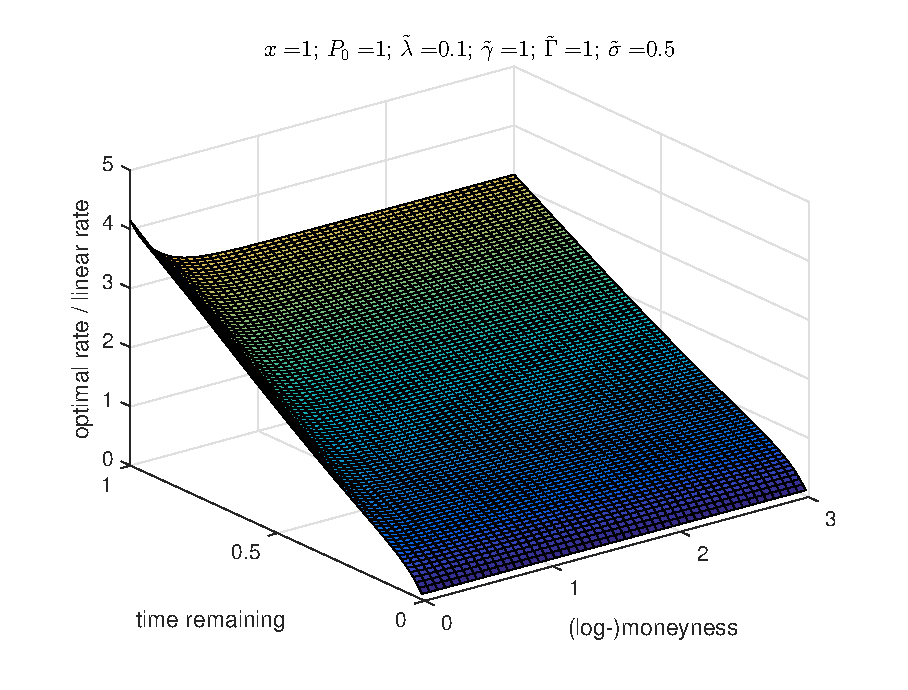
\includegraphics[]{ABM_lin.eps}
\caption{Optimal liquidation VS straight line liquidation (Arithmetic Brownian motion case)}
\label{fig:ABM_lin}
\end{figure}

\begin{figure}
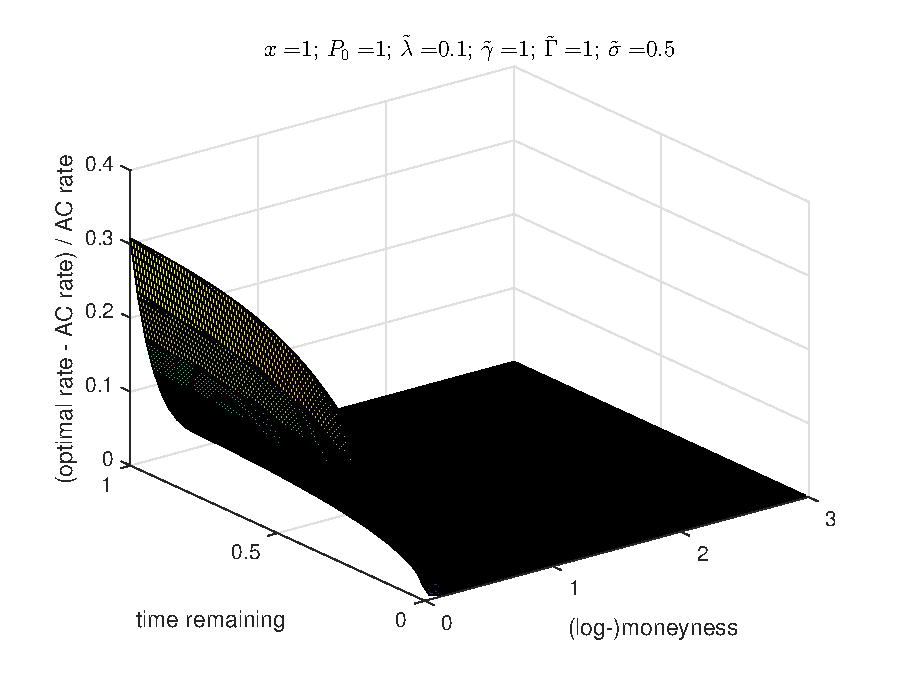
\includegraphics[]{ABM_AC.eps}
\caption{Optimal liquidation VS Almgren-Chriss liquidation (Arithmetic Brownian motion case)}
\label{fig:ABM_lin}
\end{figure}

\begin{figure}
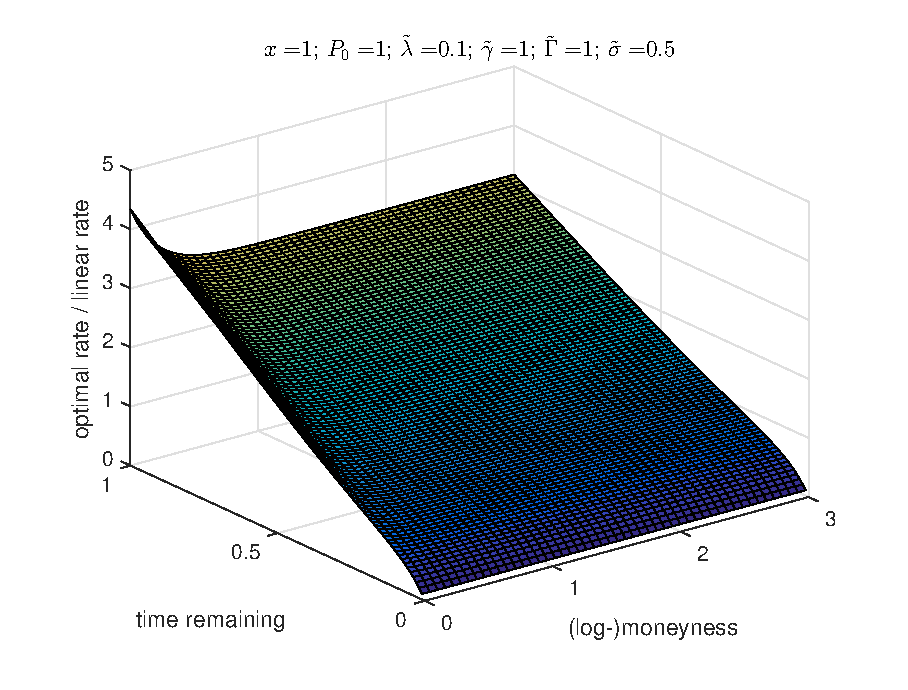
\includegraphics[]{GBM_lin.eps}
\caption{Optimal liquidation VS straight line liquidation (Geometric Brownian motion case)}
\label{fig:ABM_lin}
\end{figure}

\begin{figure}
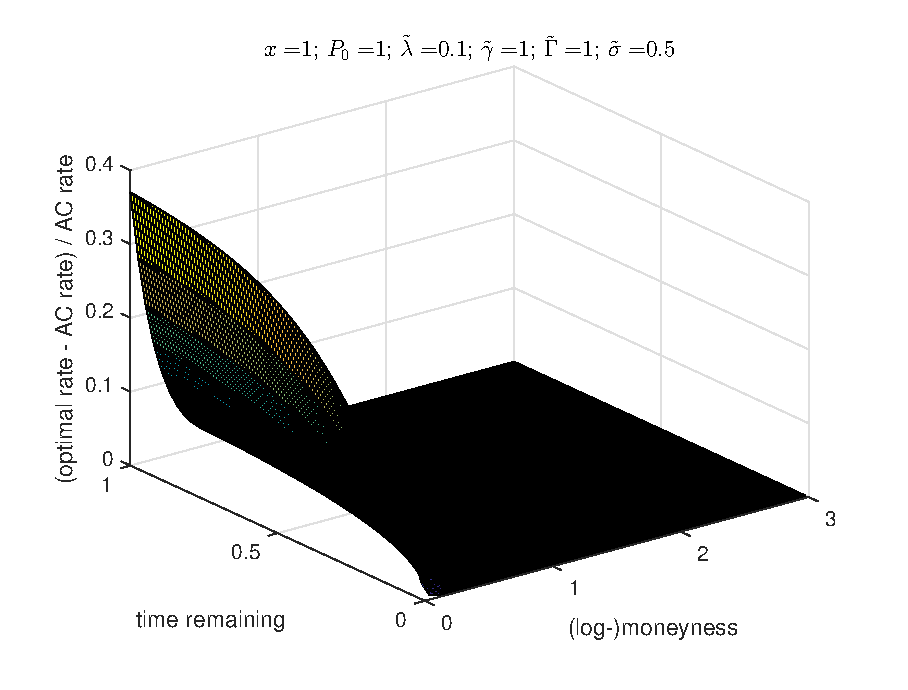
\includegraphics[]{GBM_AC.eps}
\caption{Optimal liquidation VS Almgren-Chriss liquidation (Geometric Brownian motion case)}
\label{fig:ABM_lin}
\end{figure}

% In particular, at time $t=0$ and upon assuming that $P:=P_0=S_0$, this yields
% \begin{align*}
%  \ts u_0^* &\ts= \frac{G'(T)}{G(T)} x + \frac{P}{2\lambda}\int_t^T  \frac{G(T-s)}{G(T)} \bigl[ \frac{1}{\sqrt{s}}p\bigl(f(P,P,s,0)\bigr)+\frac{1}{2}\mathcal N\bigl(f(P,P,s,0)\bigr)\bigr] \de s\\
%            &\ts= \bigl[2\lambda\beta\cosh(\beta T)+2\Gamma\sinh(\beta T)\bigr]^{-1}\\
% 					 &\ts\hspace{1.5cm}\times\Bigl[ 2\bigl[\Gamma\beta\cosh(\beta T)+\gamma\sinh(\beta T)\bigr] x\\
% 					 &\ts\hspace{2.5cm}+ P\int_0^T  \bigl[\beta\cosh(\beta (T-s))+\lambda^{-1}\Gamma\sinh(\beta (T-s))\bigr] \bigl[ \frac{\sigma}{\sqrt{s}}p\bigl(\frac{\sigma\sqrt{s}}{2} - \frac{1}{\sigma\sqrt{s}}\log\left(\frac{c}{P}\right)\bigr)\\
% 					 &\ts\hspace{9.5cm}+\frac{1}{2}\sigma^2 \mathcal N\bigl(\frac{\sigma\sqrt{s}}{2} - \frac{1}{\sigma\sqrt{s}}\log\left(\frac{c}{P}\right)\bigr)\bigr] \de s\Bigr].
% \end{align*}


% {\color{red}
% For the sake of numerical implementation (e.g. in Matlab), we express our results as follows.
% \begin{multline*}
% \ts \de_s L_s(t) = S_t\sigma^2 \Bigl[p\left(\log\left(\frac{c-P_t}{S_t}+1 \right); \frac{1}{2}\sigma^2(s-t), \sigma^2(s-t)\right)\\
%    \ts + \frac{1}{2}\left(1-\mathcal{N}\left(\log\left(\frac{c-P_t}{S_t}+1 \right); \frac{1}{2}\sigma^2(s-t), \sigma^2(s-t)\right)\right)\Bigr] \de s,
% \end{multline*}
% where $p(\cdot;\mu,\Sigma)$ and $\mathcal{N}(\cdot;\mu, \Sigma)$ are respectively the probability density function and the cumulative distribution function of a normal random variable with mean $\mu\in\mathbb{R}$ and variance $\Sigma>0$.

% With $\tau$ and $u^M$ as in the case of arithmetic Brownian motion, and further introducing the ``log-moneyness'' variable $l:=\log\left(\frac{c-P_t}{S_t}+1\right)$, we have
% \begin{align*}
% \ts u^\ast_t = u^M_t + \frac{S_t\sigma^2}{2\lambda}\int_0^\tau \frac{G(\tau-s)}{G(\tau)}\left[p(l;\frac{1}{2}\sigma^2 s, \sigma^2 s)+\frac{1}{2}(1-\mathcal{N}(l;\frac{1}{2}\sigma^2 s, \sigma^2 s))\right] \de s.
% \end{align*}

%\subsection{Geometric Brownian motion}
%Now suppose that $S$ is a standard geometric Brownian motion, i.e. $S_t:=\mathcal{E}(B)_t = \exp\left(B_t-\frac{1}{2}t\right)$ in which $B$ is a standard Brownian motion. We would like to compute $\P_t(\tau_t(y)\le s) = \P^{0,S_t}(\tau_0(y)\le s-t)$ for $y>M_t$.
%
%For simplicity, we will compute $\P^{0,x}(\tau_0(y)\le \theta)$ for $y>x$. Define $\tilde{B}_t:=B_t-\frac{1}{2}t$ and $Z_t:=\exp\left(-\frac{1}{2}\tilde{B}_t-\frac{1}{8}t\right)$. Set $\tilde\tau(z):=\inf\{t\in[0,\infty] : \tilde{B}_t = z\}$. Let $\tilde\P$ be such that $\frac{d\P}{d\tilde\P}=Z_\theta$, then by Girsanov's theorem, $\{\tilde{B}_t\}_{t\in[0,\theta]}$ is a Brownian motion under $\tilde\P$. Thus, with knowledge of the first hitting time of a standard Brownian motion,
%\begin{align*}
%& \P^{0,x}(\tau_0(y)\le \theta) = \P(\tilde\tau(\log(y/x)) \le \theta) = \tilde\E\left[Z_\theta \I_{\{\tilde\tau(\log(y/x))\le \theta\}}\right] = \tilde\E\left[Z_{\tilde\tau(\log(y/x))} \I_{\{\tilde\tau(\log(y/x))\le \theta\}}\right] \\
%=& \tilde\E\left[\exp\left(-\frac{1}{2}\log(y/x)-\frac{1}{8}\tilde\tau(\log(y/x))\right) \I_{\{\tilde\tau(\log(y/x))\le \theta\}}\right] = \int_0^\theta (y/x)^{-1/2}e^{-t/8} d_t\tilde\P(\tilde\tau(\log(y/x)) \le t) \\
%=& \int_0^\theta (y/x)^{-1/2}e^{-t/8} d_t\left(2\tilde\P(\tilde{B}_t>\log(y/x))\right) = \int_0^\theta (y/x)^{-1/2}e^{-t/8} d_t\left(2\int_{\log(y/x)}^\infty p(t,z) dz\right) \\
%=& \int_0^\theta (y/x)^{-1/2}e^{-t/8} \left(\int_{\log(y/x)}^\infty 2\partial_t p(t,z) dz\right) dt = \int_0^\theta (y/x)^{-1/2}e^{-t/8} \left(\int_{\log(y/x)}^\infty \partial^2_z p(t,z) dz\right) dt \\
%=& -\int_0^\theta (y/x)^{-1/2}e^{-t/8} \partial_z p(t,\log(y/x)) dt, \quad \textrm{ where } p(t,z):=(2\pi t)^{-1/2}\exp\left(-\frac{z^2}{2t}\right).
%\end{align*}
%Therefore, let $z:=\log(y/x)$ we have
%\begin{align*}
%& \int_K^\infty \P^{0,x}(\tau_0(y)\le \theta) dy = -\int_{\log(K/x)}^\infty \int_0^\theta e^{-z/2} e^{-t/8} \partial_z p(t,z) dt d(xe^{z}) = -x \int_0^\theta e^{-t/8} \int_{\log(K/x)}^\infty e^{z/2} \partial_z p(t,z)) dz dt \\
%=& x \int_0^\theta e^{-t/8} \left[(K/x)^{1/2} p(t,\log(K/x)) + \int_{\log(K/x)}^\infty \frac{1}{2}e^{z/2}p(t,z) dz\right] dt \\
%=& x \int_0^\theta \left[p(t,\log(K/x)-t/2) + \frac{1}{2}\int_{\log(K/x)}^\infty p(t,z-t/2) dz\right] dt.
%\end{align*}
%With $x=S_t, K=c\vee M_t=(c\vee M_t -c - S_t) + c + S_t =c-P_t+S_t$, and $\theta=s-t$, we obtain
%\begin{align*}
%& L_s(t)=S_t \int_0^{s-t} \left[ p\left(\tau,\log\left(\frac{c-P_t}{S_t}+1\right)-\tau/2 \right)+\frac{1}{2}\int_{\log\left(\frac{c-P_t}{S_t}+1\right)}^\infty p(\tau,z-\tau/2)dz \right] d\tau \\
%\Rightarrow & d_s L_s(t) = S_t\left[ p\left(s-t,\log\left(\frac{c-P_t}{S_t}+1\right)-\frac{s-t}{2} \right)+\frac{1}{2}\int_{\log\left(\frac{c-P_t}{S_t}+1\right)}^\infty p\left(s-t,z-\frac{s-t}{2}\right)dz \right] ds.
%\end{align*}
%In short, we also have an explicit formula for the optimal selling rate if $S$ is a geometric Brownian motion. 

%\subsection{It\^o Diffusion}
%If $S$ is a diffusion given by the stochastic differential equation (SDE) $dS_t = \sigma(t,S_t) dB_t$, where $\sigma$ is uniformly Lipschitz in space and $B$ is a standard Brownian motion (note that $S$ is a martingale), then the cumulative distribution function (CDF) of the first hitting time $\P^{t,x}(\tau_t(y)\le s)=:u(t,x;s,y)$ can be characterized as the bounded solution to the following linear heat equation:
%\begin{align*}
%\begin{cases}
%(\partial_t + \mathcal{L}^S)u = \partial_t u + \frac{1}{2}\sigma^2\partial^2_x u = 0, & t<s, x<y \\
%u(t,y;s,y)=1, & t<s \\
%u(s,x;s,y)=\I_{\{x=y\}}, & x<y
%\end{cases}.
%\end{align*}
%Then we can write $L_s(t) = \int_{c\vee M_t} u(t,B_t;s,y) dy$.
%
%Now that one has to solve a PDE for diffusive $S$, we can also directly obtain a PDE for $L_s(t)$. Set $u(t,x,y;s,K):=\E\left[(M_s-K)_+ \vert S_t=x, M_t=y\right]$, then $u$ solves the following linear heat equation:
%\begin{align*}
%\begin{cases}
%(\partial_t u + \mathcal{L}^S)u = \partial_t u + \frac{1}{2}\sigma^2\partial^2_x u = 0, & t<s, x<y \\
%\partial_y u(t,y,y;s,K) = 0, & t<s \\
%u(s,x,y;s,K) = (y-K)_+, & x<y
%\end{cases}
%\end{align*}
%Then we can write $L_s(t) = u(t,B_t,M_t;s,c\vee M_t)$.

%\subsection{Price floor and model assumptions}
%Our proposition also applies to the case of liquidating a positive position of an asset in the presence of a price floor, and in particular, there is a unique optimal strategy absolutely continuous with respect to time. Formally, let $P=S+(f-M)_+$ be the asset price in which $S\in\mathcal{H}^1$ is a martingale and $M_t:=\inf_{u\in[0,t]}S_u$ is the running minimum. This is the dual case of an asset of price $-P$ and a price cap at $-f$. Thus, $P_t\ge f$ with equality iff $S_t=M_t\le f$, and $E_t P_s = P_t + \E_t[(f\wedge M_t-M_s)_+]$ from the beginning of this section. Therefore, one can solve the optimal liquidation problem with a price floor by pricing fixed-strike lookback puts. In the case of $S=B$, a standard Brownian motion, the optimal selling rate is
%\begin{align*}
%r^\ast_t &= -\frac{1}{2\lambda G(T-t)}\left(-2\lambda G'(T-t) X_t + \int_t^T G(T-s)p(s-t,P_t-f) ds\right) \\
%&= -\left[2\lambda\beta\cosh(\beta (T-t))+2\Gamma\sinh(\beta (T-t))\right]^{-1} \\
%& \cdot \left(- 2\left[\Gamma\beta\cosh(\beta (T-t))+\gamma\sinh(\beta (T-t))\right] X_t + \int_t^T \left[\beta\cosh(\beta (T-s))+\lambda^{-1}\Gamma\sinh(\beta (T-s))\right] \frac{\exp{\left(-\frac{(P_t-f)^2}{2(s-t)}\right)}}{\sqrt{2\pi(s-t)}} ds \right),
%\end{align*}
%Note that the sign of the integral term is flipped.
%
%However, it makes little economic sense to interpret $\lambda r_t$ as the temporary price impact of selling $r_t dt$ units of the asset at the price floor $f$, because by definition there should be no downward price impact at the floor. In this case, one could argue that it is a trading cost from commissions or exchange fees instead of temporary price impact, but in reality, these costs are usually proportional to the total shares traded or even decreasing in trading intensities. Therefore, we think that our model is not suitable for asset liquidation in the presence of a price floor.

% references
\bibliographystyle{plainnat}
\phantomsection
\addcontentsline{toc}{section}{\refname}
\bibliography{References}

\end{document}